\documentclass[preprint,12pt]{elsarticle}

\usepackage[utf8]{inputenc}
\usepackage[T1]{fontenc}
\usepackage{amsmath,amssymb}
\usepackage{booktabs}
\usepackage{array}
\usepackage{graphicx}
\usepackage[hidelinks]{hyperref}
\usepackage{xcolor}

\emergencystretch=2em
\setlength{\textfloatsep}{22pt plus 3pt minus 4pt}
\setlength{\intextsep}{16pt plus 2pt minus 3pt}

\newcommand{\R}{\mathbb{R}}
\newcommand{\Ephys}{\mathcal{E}_{\mathrm{phys}}}
\newcommand{\Pset}{\mathcal{P}}
\newcommand{\mlu}{\operatorname{MLU}}

\begin{document}

\begin{frontmatter}

\title{Does Discrete Ricci Curvature Improve Failure-Aware Traffic
Engineering? A Controlled Comparison with Direct Scenario-Risk Optimization}

\author{Emre \"Ozt\"urk}
\ead{emre.ozturk@mku.edu.tr}
\affiliation{organization={Department of Management Information Systems,
Hatay Mustafa Kemal University}, city={Hatay}, country={T\"urkiye}}

\begin{abstract}
Discrete Ricci curvature describes structural fragility, but diagnostic
association does not establish routing value. We test the
incremental prescriptive value of negative Ollivier--Ricci curvature against
capacity-aware and outcome-aligned traffic engineering (TE). Path-based
multi-commodity flow on directed REPETITA backbones preserves capacities and
origin--destination commodities. All policies share candidate paths and
matched maximum-link-utilization (MLU) and latency budgets; one traffic matrix
tunes regularization and four remain held out. Resilience is independent
frozen-route service loss after physical-link failures, with adaptive
capacity-feasible delivery as a recovery ceiling.

On a frozen ten-topology set, curvature did not improve mean
single-link-failure delivery: relative to minimum-MLU TE, loss increased by
0.452 percentage points (topology-bootstrap 95\% CI: 0.077 to 0.935; exact
sign-flip $p=0.0625$) and path cost by 1.36\%. A direct single-link minimax
control on ten disjoint topologies reduced
worst loss relative to curvature by 2.246 points (95\% CI: 0.871 to 3.596
points; $p=0.03125$). We generalize direct control to
expected-loss, CVaR, and minimax programs for multi-link scenarios. On twelve
topologies with design/evaluation link-pair splits, CVaR(0.90) TE
reduced held-out CVaR loss relative to curvature by 1.297 points (95\% CI:
0.554 to 2.074 points; $p=0.015625$), while mean loss increased
by 0.281 points and path cost by 1.90\%. Curvature conclusions survived
path-count, MLU-slack, and laziness checks; tail gains weakened with only 40
design scenarios. Geometry is useful diagnostically,
but direct risk objectives better control the declared failure-loss tail and
make its mean--tail trade-off explicit.
\end{abstract}

\begin{keyword}
traffic engineering \sep network resilience \sep multi-commodity flow \sep
Ollivier--Ricci curvature \sep Forman--Ricci curvature \sep link failure \sep
REPETITA
\end{keyword}

\end{frontmatter}

\section{Introduction}

Traffic engineering (TE) determines how a traffic matrix is carried by a
capacitated network. Classical objectives balance load, minimize delay, or
protect the network against demand and topology changes
\cite{fortz2000,liu2014ffc}. Link failures make this problem explicitly
structural: a routing that is satisfactory in the nominal topology may lose a
large fraction of traffic before a controller converges or installs a new
configuration. Reproducible frameworks such as REPETITA therefore evaluate both
stored configurations under failure and reoptimization after failure
\cite{gay2017repetita}.

That literature has moved through increasingly explicit treatments of
uncertainty. Nominal link-weight optimization first centered on utilization and
delay; robust and oblivious formulations then protected against uncertain
demand sets \cite{applegate2003robust,wang2006cope}. Failure-aware systems added
precomputed or rapidly installed alternatives \cite{wang2010r3,liu2014ffc},
while TeaVaR introduced distributional availability risk into WAN TE
\cite{bogle2019teavar}. Recent DOTE, outcome-aware mitigation, and maximum-load
verification evaluate end-to-end behavior under demand and topology changes
rather than relying on local surrogates
\cite{perry2023dote,namyar2025mitigation,schneider2025loads}. This trajectory
makes the comparison standard for a new routing signal demanding: it should be
tested not only against nominal TE, but also against controls that directly
encode the declared failure outcome. Discrete curvature enters this history
from a different direction, as a geometric descriptor rather than an
operational objective.

Discrete Ricci curvature formalizes that geometric view of network structure.
Ollivier--Ricci curvature compares probability measures around adjacent nodes
through optimal transport \cite{ollivier2009}; Forman--Ricci curvature provides
a cheaper combinatorial alternative \cite{forman2003,samal2018}. On Internet
topologies, curvature is associated with local heterogeneity, betweenness, and
connectivity \cite{ni2015}. Across several domains it has consequently been
used as a proxy for robustness or vulnerability. These uses are diagnostic:
they ask whether a score identifies an edge with a particular structural role.
They do not by themselves show that placing the score in a routing objective
improves a network-level outcome.

This distinction matters because a curvature penalty mechanically moves traffic
away from negatively curved edges. Measuring success as ``less traffic on
negative-curvature edges'' then reuses the treatment variable as the outcome.
Such a comparison cannot tell whether more traffic is delivered when a link
actually fails, whether the same effect is available from degree or
betweenness, or whether ordinary capacity-aware TE already performs better.

We address the prescriptive question directly:

\begin{quote}
At matched utilization and latency budgets, does a discrete-curvature
regularizer improve service delivery after physical link failures beyond
minimum-MLU traffic engineering and curvature-blind structural controls?
\end{quote}

The study makes five contributions.

\begin{enumerate}
\item It formulates the comparison as path-based multi-commodity TE, retaining
OD identities, directed capacities, and a method-neutral candidate-path set.
\item It defines resilience through independent failure outcomes: frozen-route
delivered traffic and capacity-feasible delivery on the residual topology.
\item It separates development from confirmation. One traffic matrix tunes
regularization; four matrices per topology remain held out, and the primary
effect is tested with topology-level rather than link-level inference.
\item It generalizes a single-link exposure control to a scenario-risk LP for
expected loss, CVaR, and minimax loss under multi-link failures. The formulation
is an outcome-aligned control---not a claim that risk-aware TE is new.
\item It uses disjoint development, single-failure confirmation, tail
validation, and topology-plus-scenario double-failure sets. One-factor
sensitivity of both curvature and scenario-risk choices, an adaptive recovery
ceiling, and a fixed 30--69-node timing sequence probe robustness and cost.
\end{enumerate}

The confirmatory result is negative but informative: Ollivier--Ricci
regularization does not improve average single-link-failure delivery. The
observed tail-risk signal is also not unique to geometry; separately held-out
validation shows that directly optimizing the relevant failure outcome is more
effective. These findings delimit where
curvature can be useful: as a structural descriptor or hypothesis generator,
not as a substitute for a validated TE objective.

\section{Background and related work}

\subsection{Capacity-aware and failure-aware traffic engineering}

Load-balancing TE commonly minimizes maximum link utilization or optimizes link
weights against a projected traffic matrix \cite{fortz2000}. Robust and
oblivious formulations already address uncertain demands: early intradomain
work characterized the trade-off between performance on a known matrix and
robustness to a demand set, while COPE optimized for dynamic environments
\cite{applegate2003robust,wang2006cope}. Centralized systems such as B4 and SWAN
show how multi-commodity optimization, utilization, and operational path
constraints interact in wide-area networks \cite{jain2013b4,hong2013swan}.

Failure-aware systems reserve alternatives, precompute forwarding state, or
reoptimize after topology changes. R3, forward fault correction, fast segment
routing optimization, and semi-oblivious TE provide distinct points in this
design space \cite{wang2010r3,liu2014ffc,gay2017segment,kumar2018smore}. More
recent restoration-aware and black-hole-resilient systems further demonstrate
that the recovery mechanism and its failure model must be explicit
\cite{zhong2021arrow,krishnaswamy2022blastshield}. The methodological implication
is that failure performance must be measured on declared failed topologies or
traces, not inferred from a nominal structural score.

Recent systems sharpen that requirement. DOTE evaluates prediction-free WAN
TE under demand variation and random multi-link faults, while performance-aware
mitigation ranks actions by estimated end-to-end flow outcomes rather than
local or global proxy scores \cite{perry2023dote,namyar2025mitigation}. Velo
shows that worst link loads can change materially when route changes accompany
failures and develops scalable verification for the joint state space
\cite{schneider2025loads}. These systems address different control planes, but
all reinforce the distinction between a structural proxy and the operational
quantity ultimately optimized or verified.

REPETITA was designed to make such comparisons repeatable. It provides real
topologies augmented with bandwidth, delay, and traffic matrices, implements
multi-commodity-flow lower bounds and established TE algorithms, and includes
single-link-failure scenarios with and without reoptimization
\cite{gay2017repetita}. The underlying real-network corpus is derived from the
Internet Topology Zoo \cite{knight2011zoo}; related survivable-design instances
are available in SNDlib \cite{orlowski2010sndlib}. Robust validation research
also warns against evaluating a design on the same uncertainty set used to
construct it \cite{chang2017validation}. We therefore use REPETITA's data model
and failure distinction while implementing a common path-based optimization
layer for all policies. MetaOpt's adversarial analysis of production TE
heuristics provides a complementary lesson: the performance gap between a
heuristic and its outcome-aligned comparator is itself an important object of
study \cite{namyar2024metaopt}.

\subsection{Risk-aware traffic engineering}

Probabilistic failure objectives are established in TE. TeaVaR, in particular,
uses a Value-at-Risk view to trade utilization against availability under a
failure distribution \cite{bogle2019teavar}. Expected loss, conditional
value-at-risk (CVaR), and worst-case loss are therefore not novelty claims of
this paper; the scenario-based CVaR representation follows the standard
Rockafellar--Uryasev construction \cite{rockafellar2000cvar}. We use these risk
functionals as strong, outcome-aligned controls. The unresolved
question is narrower: after capacity, latency, candidate paths, and failure
information are controlled, does a topology-only geometric score retain
incremental prescriptive value? To prevent direct controls from being tested
on their own design scenarios, multi-link scenarios are deterministically
split before optimization and only the disjoint subset is used for evaluation.

\subsection{Discrete curvature as a structural score}

For a graph with metric $d$ and an $\alpha$-lazy probability measure $m_u$
around node $u$, Ollivier--Ricci curvature of edge $(u,v)$ is
\begin{equation}
  \kappa_{uv}=1-\frac{W_1(m_u,m_v)}{d(u,v)},
  \label{eq:orc}
\end{equation}
where $W_1$ is the Earth Mover's (1-Wasserstein) distance
\cite{ollivier2009}. Negative values indicate that the two local measures are
farther apart than their base nodes and frequently occur at sparse connections
between neighborhoods. Internet measurements show relationships with degree,
betweenness, connectivity, and geography \cite{ni2015}. These relationships
motivate---but do not validate---a routing penalty.

Forman--Ricci curvature is defined from cell-complex incidence and edge/node
weights \cite{forman2003}. Its graph specialization is inexpensive, and
empirical comparisons show that it overlaps with but is not equivalent to
Ollivier curvature \cite{sreejith2016forman,samal2018}. Extensions also treat
direction and other complex-network geometry \cite{saucan2019directed}. We
therefore treat Forman curvature as a separate baseline rather than an exact
surrogate for Ollivier curvature. Curvature-guided hierarchical partitioning
and routing has also appeared for heterogeneous communication networks
\cite{chiriac2026hierarchical}; its goal is scalable decomposition, whereas our
target is service loss under capacity-constrained physical failures.

\subsection{Gap addressed by this study}

Three questions are often conflated: (i) does a score correlate with a
structural property, (ii) does it predict the outcome of an actual failure, and
(iii) does optimizing that score improve routing? Our design evaluates all
routing policies on (iii) using outcomes that do not contain the policy's own
score. It also includes curvature-blind controls to determine whether an effect
is geometric or merely a consequence of regularization.

Table~\ref{tab:closest-work} makes the novelty boundary explicit. Risk-aware TE
already optimizes failure distributions, recent systems optimize or verify
end-to-end failure outcomes, and curvature already supports structural analysis
and hierarchical routing. To our knowledge, no prior study joins these lines in a
matched incremental-value test: identical candidate paths, MLU and latency
budgets, independent physical-failure outcomes, curvature-blind controls, and
direct scenario-risk optimizers are evaluated on held-out topologies and
failure pairs. The contribution is this controlled prescriptive audit and its
evidence, not a claim that CVaR, minimax optimization, or curvature is new.

\begin{table*}[t]
\centering
\caption{Closest methodological neighbors and the remaining comparison gap.}
\label{tab:closest-work}
\scriptsize
\setlength{\tabcolsep}{3pt}
\renewcommand{\arraystretch}{1.08}
\begin{tabular}{p{0.18\textwidth}p{0.23\textwidth}p{0.25\textwidth}p{0.25\textwidth}}
\toprule
Line of work & Failure or uncertainty target & Validation and scale emphasis & Boundary relative to this study \\
\midrule
TeaVaR \cite{bogle2019teavar} & Probabilistic availability--utilization trade-off using a VaR formulation & WAN failure distributions and risk-aware TE & Establishes that probabilistic risk objectives are not new; does not test the incremental value of a topology-only geometric regularizer. \\
DOTE \cite{perry2023dote} & Demand uncertainty with random multi-link faults & Stochastic optimization, learned scaling, and large-WAN evaluation & Addresses prediction-free TE quality and failure recovery, not a matched geometric-score audit. \\
MetaOpt \cite{namyar2024metaopt} & Adversarial inputs that expose heuristic performance gaps & Solver-based analysis of production TE and other heuristics & Motivates controlled incremental-value comparisons, but does not study curvature or held-out physical-failure loss. \\
Outcome-aware failure analysis \cite{namyar2025mitigation,schneider2025loads} & End-to-end mitigation quality and worst link loads under failures or route changes & Production incidents, large data centers, and ISP-scale verification & Optimizes or verifies operational outcomes directly; it does not compare those outcomes with curvature-aware routing under common budgets. \\
Curvature-guided networking \cite{ni2015,chiriac2026hierarchical} & Internet structure and curvature-guided hierarchical partitioning/routing & Structural association and scalable community decomposition & Supplies the geometric motivation, but not capacity- and demand-matched tests against direct scenario-risk controls. \\
This study & Frozen single- and double-link service loss; expected, CVaR, and worst-case risk & Four separated topology roles, held-out traffic matrices and failure pairs, topology-level inference & Estimates the residual prescriptive value of curvature after paths, MLU, latency, and failure information are controlled. \\
\bottomrule
\end{tabular}
\end{table*}


\section{Model}

\subsection{Directed network and physical links}

Let $G=(V,A)$ be a directed routing graph. Arc $a\in A$ has capacity $c_a>0$
and delay $\ell_a>0$. Reciprocal arcs belong to the same physical link
$e\in\Ephys$. A physical-link failure removes both directions. REPETITA
parallel arcs with identical delay and IGP weight are represented as one
capacity bundle; unequal-cost parallel arcs are excluded rather than
approximated.

Let $K$ denote the OD commodities. Commodity $k$ has source $s_k$, destination
$t_k$, and demand $d_k$. We generate the same $q=8$ delay-shortest simple paths
$\Pset_k$ for every method. Variable $x_{kp}\geq0$ denotes the amount of
commodity $k$ assigned to path $p$.

\subsection{Minimum-MLU stage}

Every policy first solves the same linear program:
\begin{align}
 \min_{x,U}\quad & U, \\
 \text{s.t.}\quad
 & \sum_{p\in\Pset_k}x_{kp}=d_k, &&\forall k\in K, \\
 & \sum_{k\in K}\sum_{p\in\Pset_k:a\in p}x_{kp}
      \le Uc_a, &&\forall a\in A, \\
 & x_{kp}\ge0,\quad U\ge0.
 \label{eq:mlu}
\end{align}
This produces $U^\star$. Unlike an ex-post overflow proxy, capacity is part of
the optimization and OD commodities cannot cancel at intermediate nodes.

\subsection{Matched-budget structural regularization}

For a nonnegative normalized arc score $r_a$, the second stage constrains
$U\le(1+\epsilon)U^\star$ with $\epsilon=0.02$ and minimizes
\begin{equation}
 \sum_{k,p}x_{kp}\left(
   \frac{L_p}{\widetilde L}+\lambda
   \frac{R_p}{\widetilde R}\right),
 \qquad
 L_p=\sum_{a\in p}\ell_a,\quad R_p=\sum_{a\in p}r_a,
 \label{eq:risk}
\end{equation}
where tildes denote within-instance scale factors. We test:

\begin{itemize}
\item endpoint-degree product;
\item edge betweenness;
\item negative Forman curvature, $r_e=[-F_e]_+$;
\item negative Ollivier curvature, $r_e=[-\kappa_e]_+$;
\item a seeded random-placebo score.
\end{itemize}

Curvature is computed on the undirected physical projection and assigned to
both directed arcs. Ollivier curvature is calculated exactly with $\alpha=0.5$
by solving the local Earth Mover's Distance problem. For each policy,
$\lambda\in\{0.03,0.1,0.3,1,3,10,30\}$ is selected using training traffic
matrix 0000 only. A setting is eligible if training mean path cost is no more
than 5\% above the minimum-MLU reference; among eligible settings, the one with
minimum score exposure is selected.

\subsection{Direct scenario-risk controls}

The single-link control was designed after inspecting the first confirmatory
secondary outcome and frozen before evaluation on a third, disjoint topology
set. The submission upgrade generalizes it to an explicit design-scenario set
$S$. Let $h_{skp}=1$ if path $p$ intersects one or more physical links in
failure scenario $F_s$, and zero otherwise. Counting the path once prevents a
two-link scenario from double-counting traffic whose path contains both links.
Normalized frozen loss is
\begin{equation}
 L_s(x)=\frac{1}{D}\sum_{k,p}h_{skp}x_{kp},\qquad D=\sum_k d_k.
 \label{eq:scenario-loss}
\end{equation}
Within the same MLU and mean-path-cost budgets, the second lexicographic stage
optimizes one of
\begin{align}
 &\sum_{s\in S}\pi_s L_s(x), &&\text{expected loss},\\
 &\eta+\frac{1}{1-\beta}\sum_{s\in S}\pi_s\xi_s,
   \quad \xi_s\ge L_s(x)-\eta,\ \xi_s\ge0, &&\text{CVaR}_{\beta},\\
 &Z,\quad L_s(x)\le Z\quad\forall s, &&\text{minimax loss}.
 \label{eq:scenario-risk}
\end{align}
We set $\beta=0.90$ and use uniform $\pi_s$ in the design set. A third stage
minimizes path cost without worsening the attained risk. The original
single-link tail control is exactly the minimax case in which each $F_s$
contains one physical link. These objectives test whether any apparent benefit
is unique to curvature or follows more directly from optimizing the outcome.

\subsection{Optimization procedure, guarantees, and size}

For each topology and traffic matrix, the scenario-risk procedure is:

\begin{enumerate}
\item construct one method-neutral candidate-path catalog and solve exact
minimum MLU;
\item impose the common MLU allowance and the explicit mean-path-cost limit;
\item build the binary scenario--path matrix $H=[h_{skp}]$ from design
scenarios only;
\item minimize expected loss, CVaR, or maximum loss over this common feasible
set;
\item fix the attained risk value within numerical tolerance and minimize mean
path cost; and
\item evaluate the installed routing only on held-out traffic matrices and
failure scenarios. Adaptive residual delivery is solved separately and is
never an optimization target of a frozen policy.
\end{enumerate}

This construction gives two useful guarantees. First, single-link minimax is
not a separate heuristic: it is the special case of Eq.~\eqref{eq:scenario-risk}
with singleton $F_s$ and the maximum-loss functional. Second, let
$\mathcal{F}$ be the common path-flow feasible set after fixing the MLU and
latency allowances, and let $R_S$ be any of the three declared design-set risk
functionals. If $x_S^*=\arg\min_{x\in\mathcal{F}}R_S(x)$, then
$R_S(x_S^*)\le R_S(x)$ for every feasible curvature or structural policy $x$.
This design-set dominance is immediate from optimality; it supplies no
held-out guarantee, which is why the evaluation scenario set is disjoint.

Let $P$ be the number of path-flow variables, $A$ the number of directed arcs,
$K$ the number of commodities, and $S$ the number of explicit scenarios. The
expected-loss LP uses $P+1$ variables (flows and MLU), minimax uses $P+2$, and
CVaR uses $P+S+2$ (including $\eta$ and $S$ excess variables). The CVaR and
minimax risk stages contain $K$ flow-conservation equalities and at most
$A+S+2$ inequalities before bounds; fixing optimal risk for the latency
tie-break adds one inequality. The scenario--path matrix has at most $SP$
nonzeros. Thus the explicit formulation is polynomial in the supplied
path--scenario representation; the empirical timing study reports where this
representation remains tractable rather than claiming Internet-scale control.

\section{Failure outcomes and experimental design}

\subsection{Independent outcomes}

For failure set $F\subseteq\Ephys$, frozen-route delivered fraction is
\begin{equation}
 \mathrm{Delivery}_{\mathrm{frozen}}(F)=
 \frac{1}{\sum_kd_k}
 \sum_k\sum_{p:p\cap F=\varnothing}x_{kp}.
 \label{eq:frozen}
\end{equation}
The primary outcome is service loss,
$1-\mathrm{Delivery}_{\mathrm{frozen}}$, averaged over every physical
single-link failure and all held-out matrices.

For adaptive delivery, failed links are removed from the common candidate-path
catalog and a residual LP first maximizes capacity-feasible delivered traffic.
Only after the maximum delivery is fixed is policy cost used as a tie-break.
This lexicographic order prevents a method from receiving credit for renaming
its own structural score as resilience.

\subsection{REPETITA data and separation of roles}

We use the REPETITA `2016TopologyZooUCL\_inverseCapacity` dataset at repository
commit `60e679c`. Directed capacities, delays, and OD directions are preserved.
Ten development topologies were used to debug the protocol and are excluded
from confirmatory inference. Before viewing outcomes, a second set of ten
strongly connected topologies (17--23 nodes) and the implementation hashes were
frozen. Matrix 0000 tunes $\lambda$; matrices 0001--0004 are held out.

The confirmatory topologies are Aconet, Easynet, Noel, Belnet2010, Garr200109,
Fccn, Packetexchange, GtsRomania, Fatman, and Nextgen. Full inclusion rules,
exclusions, hashes, and the analysis decision are retained with the artifact.

After the direct tail-risk control was designed, a third set of ten previously
unused topologies was frozen for its primary comparison with ORC: Claranet,
HiberniaUk, Nordu2010, Spiralight, Garr199901, Grena, HostwayInternational,
Marwan, Peer1, and Rhnet. No outcome on this set was viewed before its protocol
and implementation hashes were recorded.

For multi-failure validation, a fourth, previously unused set of twelve
topologies was frozen: Sago, Pacificwave, Ibm, Highwinds, Internetmci, Restena,
Marnet, BtAsiaPac, Harnet, Bandcon, HiberniaUs, and Azrena. All unordered pairs
of physical links form the scenario universe. A SHA-256 hash of topology and
sorted link-pair labels assigns each scenario to a design or evaluation set;
the 160 smallest hashes per set are retained when necessary. The assignment
uses no curvature, traffic outcome, or routing solution. Matrices 0001--0004
and every evaluation scenario remain hidden from all scenario-risk optimizers.

Before running additional robustness checks, we fixed a separate sensitivity
protocol. Holding the same evaluation pairs constant, it changes CVaR level to
$\beta\in\{0.80,0.95\}$ at 160 design scenarios and changes the hash-ordered
design budget to 40 or 80 scenarios at $\beta=0.90$. These checks are labeled
post-upgrade sensitivity rather than new confirmatory tests. Adaptive recovery
is computed on the first 40 hash-ordered evaluation pairs per topology and all
four held-out matrices; this cost-limited sample is identical for every score
and frozen policy comparison.

Table~\ref{tab:topologies} summarizes the confirmatory instances and the number
of independent single-link failure cases used for each topology.

\begin{table*}[t]
\centering
\caption{Held-out confirmatory REPETITA instances. Failure cases equal four test traffic matrices times all physical single-link failures. Parallel bundles contain only equal-delay, equal-IGP-weight arcs.}
\label{tab:topologies}
\small
\resizebox{\textwidth}{!}{%
\begin{tabular}{lrrrrrrr}
\toprule
Topology & Nodes & Directed arcs & Physical links & Bundles & OD pairs & Failure cases & $\lambda_{\mathrm{ORC}}$ \\
\midrule
Aconet & 23 & 62 & 31 & 0 & 506 & 124 & 1 \\
Easynet & 19 & 52 & 26 & 6 & 342 & 104 & 0.3 \\
Noel & 19 & 50 & 25 & 0 & 342 & 100 & 1 \\
Belnet2010 & 22 & 50 & 25 & 10 & 462 & 100 & 0.3 \\
Garr200109 & 22 & 48 & 24 & 0 & 462 & 96 & 0.03 \\
Fccn & 23 & 50 & 25 & 4 & 506 & 100 & 1 \\
Packetexchange & 21 & 54 & 27 & 0 & 420 & 108 & 0.3 \\
GtsRomania & 21 & 48 & 24 & 0 & 420 & 96 & 0.3 \\
Fatman & 17 & 42 & 21 & 0 & 272 & 84 & 1 \\
Nextgen & 17 & 38 & 19 & 2 & 272 & 76 & 1 \\
\bottomrule
\end{tabular}
}
\end{table*}


\subsection{Inference}

The experimental unit is the topology. For topology $g$, the primary paired
effect is
\begin{equation}
 \Delta_g=L_{\mathrm{ORC},g}-L_{\mathrm{MLU},g},
\end{equation}
where $L$ is mean frozen-route service loss across all held-out matrices and
physical single-link failures. A negative value favors ORC. The frozen primary
test is an exact two-sided sign-flip permutation test at $\alpha=0.05$.
We report the equal-topology mean and a topology-cluster bootstrap confidence
interval \cite{efron1979bootstrap}. Links are not treated as independent
observations. Secondary policy-vs-MLU tests use Holm correction
\cite{holm1979}.

The frozen multi-failure primary endpoint is topology-level CVaR(0.90) across
the Cartesian product of four held-out traffic matrices and held-out
double-link failures. Its paired contrast is double-failure CVaR TE minus ORC;
negative values favor the direct risk method. We again report an equal-topology
mean, median, topology-cluster bootstrap interval, exact two-sided sign-flip
test, and better/worse/tied counts. Mean and maximum loss, comparisons with MLU,
and adaptive recovery are secondary; Holm correction is applied within each
secondary outcome family.

\section{Results}

\subsection{Confirmatory average-failure result}

Table~\ref{tab:confirmatory} reports the held-out topology-clustered effects.
The ORC point estimate is in the harmful direction: mean failure loss is 0.452
percentage points higher than minimum MLU, and mean path cost is 1.36\% higher.
The exact primary $p$-value is 0.0625; therefore, under the frozen decision rule,
we do not reject the null. This is evidence of no demonstrated improvement, not
an equivalence conclusion. The percentile bootstrap interval and exact
sign-flip test differ at the 5\% boundary because only ten topology clusters are
available and the paired effects are skewed; the decision follows the frozen
exact test rather than selecting the more favorable inferential summary.

\begin{table}[t]
\centering
\caption{Confirmatory frozen-route service-loss effects relative to minimum
MLU. Positive values are worse. Confidence intervals resample topologies. Holm
$p$ applies to the secondary five-policy family; the preregistered ORC primary
test uses the raw exact $p=0.0625$.}
\label{tab:confirmatory}
\begin{tabular}{lrrrr}
\toprule
Policy & Mean $\Delta$ (pp) & 95\% CI (pp) & Path cost & Holm $p$ \\
\midrule
Degree & +0.270 & [-0.094, +0.782] & +1.17\% & 0.8438 \\
Betweenness & +0.205 & [-0.159, +0.717] & +1.30\% & 0.8438 \\
Forman--Ricci & +0.397 & [+0.123, +0.707] & +2.28\% & 0.2344 \\
Ollivier--Ricci & +0.452 & [+0.077, +0.935] & +1.36\% & 0.2500 \\
Random placebo & +0.197 & [-0.089, +0.518] & +2.70\% & 0.8438 \\
\bottomrule
\end{tabular}
\end{table}

No secondary policy survives family-wise correction. Importantly, neither
curvature score improves mean service loss. A structural penalty can change
where traffic is carried while leaving the independent delivery outcome
unchanged or worse. Figure~\ref{fig:paired} displays the topology-level
heterogeneity behind this mean effect and the frozen exact-test result.

\begin{figure}[t]
\centering
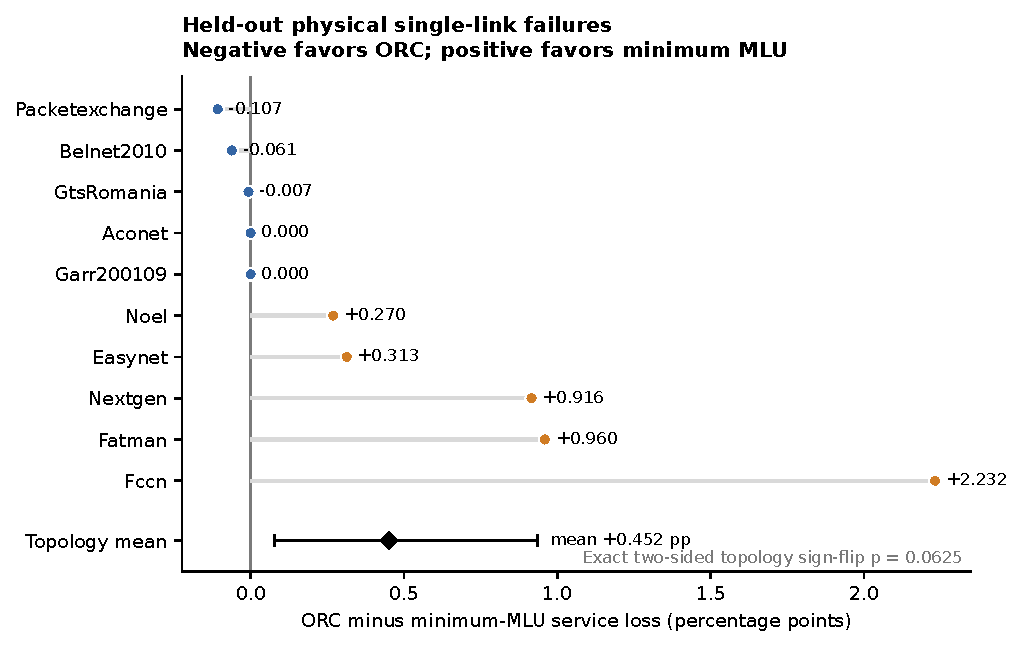
\includegraphics[width=0.94\linewidth]{figures/fig1_confirmatory_paired_effects.pdf}
\caption{Topology-level confirmatory effects for Ollivier--Ricci regularization
relative to minimum MLU. Positive values indicate greater frozen-route service
loss under exhaustive physical single-link failures. The diamond and interval
show the equal-topology mean and topology-cluster bootstrap 95\% confidence
interval.}
\label{fig:paired}
\end{figure}

\subsection{Held-out worst-failure validation}

The first confirmatory set suggested a heterogeneous worst-failure signal, so
the direct tail-robust control was designed and frozen for a new held-out test.
On that third set, tail-robust reduced worst-failure loss relative to ORC by
2.246 percentage points (bootstrap 95\% CI: -3.596 to -0.871; exact two-sided
sign-flip $p=0.03125$). It was better on six, worse on two, and tied on two
topologies. Mean failure-loss difference was -0.103 points ($p=0.5078$), and
path-cost difference was -0.433\% ($p=0.6016$); neither was detected as
non-zero.

Relative to minimum MLU, tail-robust reduced worst loss by 2.543 points
(CI: -3.661 to -1.333; $p=0.0078$), while mean loss was essentially unchanged
(+0.012 points; $p=0.7891$) and path cost rose by 1.70\%. The result resolves the
mechanism on held-out data: the tail benefit is not unique to curvature. A
linear objective that represents frozen-route failure exposure directly is
more effective. Figure~\ref{fig:tail} shows the topology-wise trajectories and
their equal-topology means under the three policies.

\begin{figure}[t]
\centering
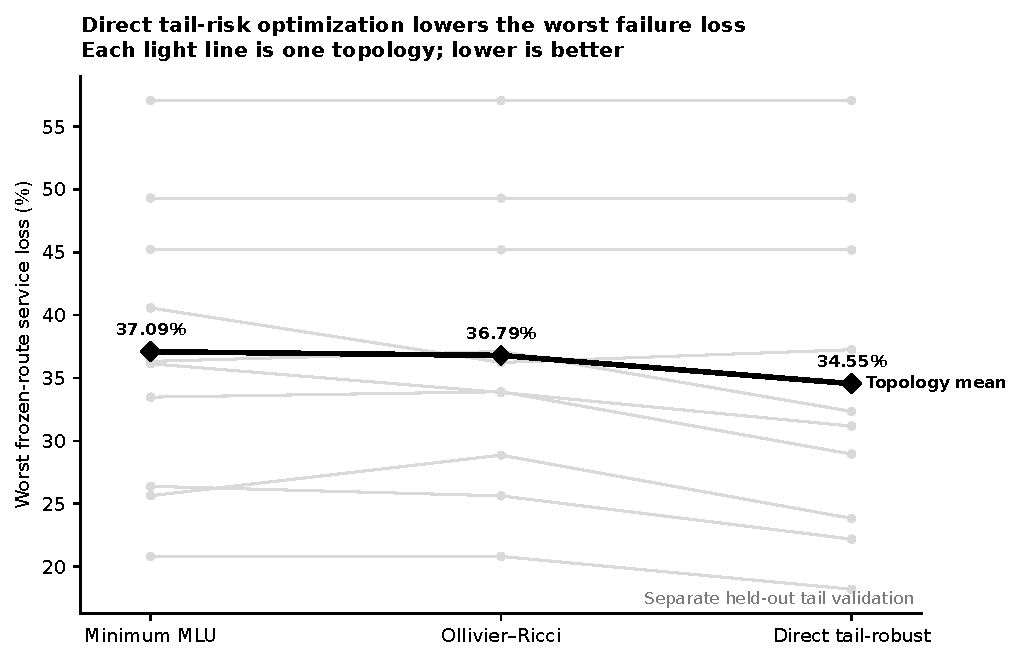
\includegraphics[width=0.94\linewidth]{figures/fig2_tail_robust_slope.pdf}
\caption{Held-out validation of worst-failure service loss on a third topology
set. Each light line represents one topology under the three policies; the dark
line is the equal-topology mean. The direct tail-robust LP reduces worst loss
more consistently than the curvature regularizer.}
\label{fig:tail}
\end{figure}

\subsection{Held-out double-failure scenario risk}

The scenario-risk extension was evaluated on twelve further topologies. Design
and evaluation link pairs were disjoint, and the evaluation pairs were never
provided to an optimizer. The frozen primary contrast supported the direct
risk control: relative to ORC, double-failure CVaR TE reduced held-out
CVaR(0.90) service loss by 1.297 percentage points (topology-cluster bootstrap
95\% CI: -2.074 to -0.554; exact two-sided sign-flip $p=0.015625$). It was
better on seven, worse on three, and tied on two topologies.
Figure~\ref{fig:double} shows that this mean is supported by seven negative
topology-level effects rather than by one extreme instance.

This tail improvement is not a free average-loss improvement. Relative to ORC,
the CVaR policy's mean loss was 0.281 points higher (95\% CI: +0.044 to +0.543;
raw $p=0.0664$) and mean path cost was 1.90\% higher. Relative to minimum MLU,
its CVaR improvement was 0.881 points (CI: -1.474 to -0.283; raw $p=0.0215$,
Holm-adjusted $p=0.0645$), while mean loss increased by 0.648 points
(Holm-adjusted $p=0.0234$) and path cost by 3.76\%. The formulation therefore
does what its objective declares---moves mass out of the upper loss tail---but
does not dominate on the mean.

Table~\ref{tab:double} also shows that the simpler single-link minimax control
generalizes strongly to unseen double failures. It reduced CVaR relative to ORC
by 1.353 points (Holm-adjusted $p=0.0156$) and worst loss by 2.319 points, with
slightly lower path cost. Expected-loss optimization did not reduce the tail.
The comparative mechanism is consequently broader than one new LP: direct
failure exposure is a more useful prescriptive signal than curvature in these
benchmarks, and the chosen risk functional determines which part of the loss
distribution improves.

\begin{table*}[t]
\centering
\caption{Held-out double-link-failure effects relative to ORC over twelve new
topologies. Negative values favor the candidate. CVaR intervals resample
topologies. The double-CVaR comparison is the frozen primary test and uses its
raw exact $p$; other adjusted values use Holm correction within the CVaR
secondary family.}
\label{tab:double}
\small
\resizebox{\textwidth}{!}{%
\begin{tabular}{lrrrrr}
\toprule
Candidate & CVaR $\Delta$ (pp) & 95\% CI (pp) & Mean $\Delta$ (pp) & Path cost & $p$ \\
\midrule
Single-link minimax & -1.353 & [-2.172, -0.635] & -0.272 & -0.84\% & 0.0156 \\
Double expected loss & -0.261 & [-0.839, +0.301] & -0.515 & -0.21\% & 0.4082 \\
Double CVaR(0.90) & -1.297 & [-2.074, -0.554] & +0.281 & +1.90\% & 0.0156$^{*}$ \\
Double minimax & -1.009 & [-1.838, -0.223] & -0.126 & +0.53\% & 0.0938 \\
\bottomrule
\end{tabular}
}

\footnotesize $^{*}$Frozen primary raw exact $p$; no selection across policies.
\end{table*}

\begin{figure}[t]
\centering
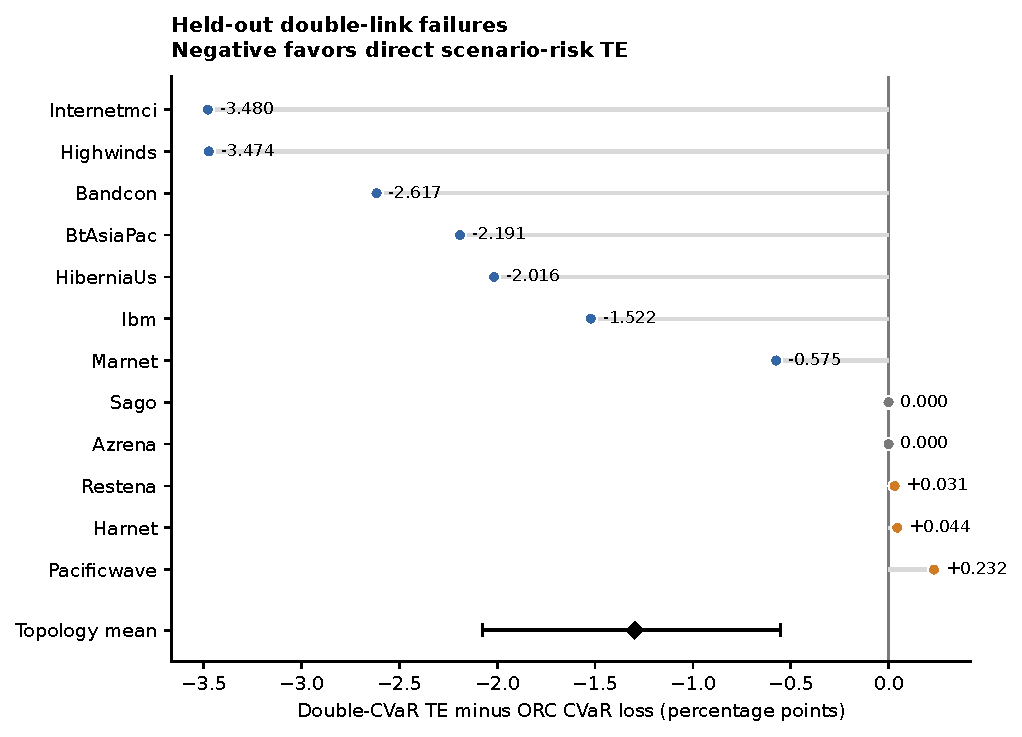
\includegraphics[width=0.94\linewidth]{figures/fig3_double_failure_cvar.pdf}
\caption{Topology-level primary effects for double-failure CVaR TE relative to
ORC on held-out link-pair scenarios. Negative values indicate lower CVaR(0.90)
service loss under the direct scenario-risk policy.}
\label{fig:double}
\end{figure}

\subsection{Sensitivity, feasibility, and runtime}

The confirmatory ORC-versus-MLU conclusion is insensitive to every frozen
one-factor change (Table~\ref{tab:sensitivity}). ORC's topology-mean
single-failure loss remains higher under $q=4$ and $q=16$ paths, zero and 5\%
MLU slack, and $\alpha=0.25$ and $0.75$. Effect magnitudes range from +0.442 to
+0.522 percentage points; no setting reverses the conclusion or removes its
path-cost increase.

\begin{table}[t]
\centering
\caption{Frozen one-factor sensitivity of ORC minus minimum-MLU mean
single-link service loss. Positive values are worse for ORC.}
\label{tab:sensitivity}
\small
\begin{tabular}{lrrr}
\toprule
Condition & Mean $\Delta$ (pp) & 95\% CI (pp) & Path cost \\
\midrule
$q=4$ & +0.522 & [+0.155, +0.942] & +1.83\% \\
$q=16$ & +0.452 & [+0.079, +0.941] & +1.56\% \\
MLU slack 0\% & +0.442 & [+0.081, +0.894] & +1.32\% \\
MLU slack 5\% & +0.465 & [+0.075, +0.968] & +1.43\% \\
ORC $\alpha=0.25$ & +0.452 & [+0.080, +0.930] & +1.36\% \\
ORC $\alpha=0.75$ & +0.452 & [+0.082, +0.937] & +1.36\% \\
\bottomrule
\end{tabular}
\end{table}

The constructive double-failure result is also stable to CVaR level and to a
moderate reduction in design scenarios (Table~\ref{tab:scenario-sensitivity}).
At 160 design scenarios, both $\beta=0.80$ and $0.95$ retain a lower held-out
CVaR(0.90) than ORC. Reducing the design budget to 80 retains a -1.100-point
effect; at 40 scenarios the estimate remains negative (-0.310 points) but its
interval crosses zero. The attenuation is operationally informative: direct
risk control needs adequate scenario coverage and is not a free consequence of
the LP form. Every condition also retains a small mean-loss and path-cost
penalty, so none establishes distribution-wide dominance.

\begin{table*}[t]
\centering
\caption{One-factor sensitivity of held-out double-failure CVaR TE relative to ORC. Negative CVaR differences favor direct risk control. The main condition is confirmatory; the other rows are protocol-fixed robustness checks.}
\label{tab:scenario-sensitivity}
\small
\resizebox{\textwidth}{!}{%
\begin{tabular}{lrrrrr}
\toprule
Condition & $\beta$ & Design scenarios & CVaR(0.90) $\Delta$ (pp) & 95\% CI (pp) & Mean $\Delta$ / path cost \\
\midrule
Main & 0.90 & up to 160 & -1.297 & [-2.074, -0.554] & +0.281 / +1.90\% \\
CVaR level & 0.80 & up to 160 & -1.343 & [-2.193, -0.490] & +0.126 / +1.59\% \\
CVaR level & 0.95 & up to 160 & -1.212 & [-2.056, -0.393] & +0.253 / +1.94\% \\
Scenario budget & 0.90 & up to 40 & -0.310 & [-1.169, +0.528] & +0.278 / +1.16\% \\
Scenario budget & 0.90 & up to 80 & -1.100 & [-1.827, -0.398] & +0.299 / +1.72\% \\
\bottomrule
\end{tabular}
}
\end{table*}


Adaptive recovery materially lowers loss but does not erase the frozen-routing
comparison (Table~\ref{tab:adaptive}). The capacity-feasible ceiling reduces
equal-topology mean loss from about 20.3--20.9 points under the stored policies
to 12.210 points, leaving an 8.117--8.713-point recoverable gap. On these same
adaptive scenarios, topology-level mean Spearman association with residual
loss is $+0.428$ for Ollivier risk (bootstrap 95\% CI: $+0.316$ to $+0.548$),
$+0.305$ for Forman risk, $+0.182$ for degree risk, and $+0.551$ for
betweenness. Betweenness is therefore the strongest of the four descriptors;
the adaptive association is structural but not uniquely geometric.

\begin{table*}[t]
\centering
\caption{Frozen routing and the capacity-feasible adaptive recovery ceiling on the same 40 held-out double-failure pairs per topology and four test matrices. Values are equal-topology means. Recoverable gap is frozen mean loss minus adaptive mean loss.}
\label{tab:adaptive}
\small
\resizebox{\textwidth}{!}{%
\begin{tabular}{lrrrr}
\toprule
Routing state & Mean loss (pp) & CVaR(0.90) (pp) & Maximum loss (pp) & Recoverable gap (pp) \\
\midrule
Adaptive capacity-feasible ceiling & 12.210 & 30.794 & 39.517 & --- \\
Frozen minimum MLU & 20.328 & 38.245 & 45.386 & 8.117 \\
Frozen Ollivier--Ricci & 20.332 & 38.785 & 45.747 & 8.121 \\
Frozen single-link minimax & 20.478 & 37.593 & 44.070 & 8.267 \\
Frozen double-failure CVaR & 20.923 & 37.536 & 44.883 & 8.713 \\
\bottomrule
\end{tabular}
}
\end{table*}


The twelve-topology double-failure run required 1,384~s wall time on a
single-process Windows workstation with an Intel Core i9-13900H and 15.7~GB
RAM. Across topologies, CVaR solves accounted for 155~s, adaptive recovery for
324~s, and exhaustive held-out evaluation for 432~s. Python allocator peaks do
not include native HiGHS memory and are therefore reported only as lower bounds.

The fixed $q=4$ feasibility sequence (Table~\ref{tab:runtime}) shows that path
variables and commodity count are more informative than node count alone. Four
instances through 69 nodes solved successfully; Surfnet was the slowest at
89.4~s for 9,720 path variables. Garr201112 was retained in the fixed sequence
but rejected by the lossless parser because it contains unequal-cost parallel
arcs. We report this boundary rather than collapsing the arcs or substituting a
more favorable topology.

\begin{table*}[t]
\centering
\caption{Fixed scalability sequence, matrix 0000 and $q=4$. Total includes
parsing, paths, ORC, tuning, and four final policies. Python peak excludes
native solver allocations.}
\label{tab:runtime}
\small
\resizebox{\textwidth}{!}{%
\begin{tabular}{lrrrrrrl}
\toprule
Topology & Nodes & Commodities & Path vars. & Paths (s) & CVaR (s) & Total (s) & Python peak \\
\midrule
GtsHungary & 30 & 867 & 1,794 & 0.81 & 4.91 & 6.98 & 21.2 MB \\
Geant2012 & 40 & 1,556 & 6,153 & 12.82 & 16.74 & 52.60 & 46.4 MB \\
Surfnet & 50 & 2,450 & 9,720 & 22.54 & 32.28 & 89.40 & 83.1 MB \\
Garr201112 & 61 & --- & --- & --- & --- & --- & unsupported arcs \\
Latnet & 69 & 4,683 & 11,026 & 19.51 & 10.50 & 47.86 & 80.5 MB \\
\bottomrule
\end{tabular}
}
\end{table*}

\section{Discussion}

\subsection{Structural diagnosis is not routing utility}

Negative curvature often highlights edges between dissimilar neighborhoods.
That may be useful for visualization, topology auditing, or generating failure
hypotheses. Routing, however, is constrained by directed capacity, the traffic
matrix, alternate paths, and the operational objective. A structural score that
correlates with failure impact need not produce a better flow allocation when
inserted as a penalty.

The controlled baselines expose this gap. Curvature regularization consumes
latency budget and changes path allocation, yet it does not improve the average
held-out delivery outcome. The direct tail objective also explains why reduced
flow on a selected structural class is insufficient evidence: if worst-link
exposure is the actual concern, it can be represented and optimized without a
geometric surrogate. The held-out double-failure study extends this conclusion:
single-link exposure control transfers to compound failures, while explicit
CVaR control shifts the upper tail at an observable mean-loss cost.

\subsection{Implications for curvature-aware networking}

Our results do not imply that discrete curvature has no networking value. They
support narrower uses and stronger validation requirements:

\begin{itemize}
\item Curvature may serve as a low-information structural feature when traffic
and capacity data are unavailable.
\item Predictive claims should compare curvature with degree, betweenness, and
placebo scores on held-out failure outcomes.
\item Prescriptive claims should compare curvature-aware routing with objectives
that directly optimize mean loss, worst loss, or a declared risk measure.
\item Risk-aware claims should report the entire mean--tail--path-cost trade-off;
improving CVaR is not evidence of first-order stochastic dominance.
\item Any computational shortcut from Forman to Ollivier curvature should report
screening recall and should not describe uncomputed edges as exact ORC.
\end{itemize}

\subsection{Limitations}

The experiments use candidate-path multi-commodity flow rather than packet-level
queues or a hardware testbed. Frozen delivery models the interval before route
replacement; adaptive delivery models an ideal capacity-feasible controller and
does not include detection or update delay. REPETITA traffic matrices and
capacities are benchmark data rather than live operator telemetry. The
first confirmatory and tail-validation sets each contain ten topologies, while
the double-failure set contains twelve; these cluster counts still limit power
for heterogeneity analysis. The tail-risk control was designed adaptively,
although its reported effects were subsequently tested on disjoint frozen
topology and scenario sets. Uniform design-scenario probabilities are a stress
model, not estimates of operator-specific joint failure probabilities. The
scenario-budget sensitivity shows that 40 design pairs are insufficient for a
precise held-out tail gain, and the largest supported fixed timing instance has
69 nodes; the evidence therefore supports tractability on these backbone
benchmarks, not Internet-scale or real-time deployment.

These limitations bound the claims. We report delivered traffic and utilization,
not packet loss, jitter, controller convergence, or ``self-healing.''

\section{Conclusion}

This study asks a prescriptive question that structural network geometry alone
cannot answer: does curvature improve routing under actual link failures? In a
matched-budget, held-out REPETITA experiment, Ollivier--Ricci regularization did
not improve average single-link-failure service delivery beyond minimum-MLU TE.
An apparent worst-failure benefit was exceeded by a direct tail-robust linear
program at comparable path cost. On a fourth set with held-out double-link
scenarios, direct CVaR optimization reduced upper-tail loss relative to ORC,
although it increased mean loss, and the single-link minimax control also
generalized. The tail effect persisted across CVaR levels but weakened under a
40-scenario design budget; ideal adaptive recovery left a substantial gap
between stored and residual-capacity routing. The central lesson is
methodological and operational: curvature
can describe a network, but resilience must be evaluated with independent
failures, and routing claims must survive comparison with objectives that
directly represent the desired outcome and its trade-offs.

\section*{Data and code availability}

The implementation, unit tests, frozen protocols, change log, exact JSON
outputs, and scripts used to generate every table and figure are assembled as a
versioned reproducibility artifact available at
\url{https://github.com/emreozi/failure-aware-ricci-te}. A new archival version
containing the submission-upgrade outputs will be deposited on Zenodo and its
DOI inserted before submission. The external REPETITA source commit and dataset
path are recorded in the artifact; benchmark data retain their original
attribution and license \cite{gay2017repetita}.

\section*{CRediT authorship contribution statement}

Emre Öztürk: Conceptualization, Methodology, Software, Validation, Formal
analysis, Investigation, Data curation, Visualization, Writing---original
draft, Writing---review and editing.

\section*{Declaration of competing interest}

The author declares no competing financial or personal interests.

\section*{Declaration of generative AI and AI-assisted technologies in the
writing process}

During preparation of this work, the author used Anthropic Claude and OpenAI
Codex for language editing, code-review assistance, manuscript organization,
and preparation of reproducibility materials. After using these tools, the
author reviewed and edited the content as needed and takes full responsibility
for the content of the published article.

\bibliographystyle{elsarticle-num}
\bibliography{references}

\end{document}
